\documentclass{article}
\usepackage{amsmath}    
\usepackage{tikz}

\begin{document}

\begin{figure}[ht]
    \centering
    \begin{subfigure}{0.29\textwidth}
        \centering
        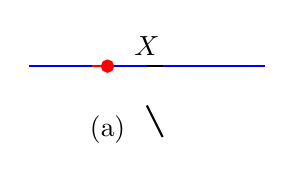
\begin{tikzpicture}[thick,scale=1]
            \draw (0,-0.5) -- ++(0.2,-0.4);
            \draw[color=blue] (-1.5,0) -- ++(3,0);
            \draw[color=red] (-0.5,0) -- ++(-0.2,0);
            \draw (0,0) -- ++(0.2,0);
            \filldraw [red] (-0.5,0) circle (2pt);
            \node [below] at (-0.5,-0.5) {(a)};
            \node [above] at (0,0) {$X$};
        \end{tikzpicture}
        \label{fig:a}
    \end{subfigure}
    \begin{subfigure}{0.29\textwidth}
        \centering
        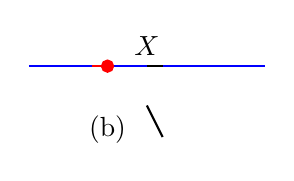
\begin{tikzpicture}[thick,scale=1]
            \draw (0,-0.5) -- ++(0.2,-0.4);
            \draw[color=blue] (-1.5,0) -- ++(3,0);
            \draw[color=red] (-0.5,0) -- ++(-0.2,0);
            \draw (0,0) -- ++(0.2,0);
            \filldraw [red] (-0.5,0) circle (2pt);
            \node [below] at (-0.5,-0.5) {(b)};
            \node [above] at (0,0) {$X$};
        \end{tikzpicture}
        \label{fig:b}
    \end{subfigure}
    \begin{subfigure}{0.29\textwidth}
        \centering
        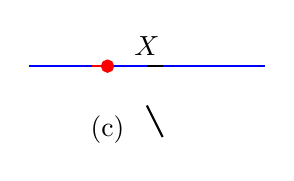
\begin{tikzpicture}[thick,scale=1]
            \draw (0,-0.5) -- ++(0.2,-0.4);
            \draw[color=blue] (-1.5,0) -- ++(3,0);
            \draw[color=red] (-0.5,0) -- ++(-0.2,0);
            \draw (0,0) -- ++(0.2,0);
            \filldraw [red] (-0.5,0) circle (2pt);
            \node [below] at (-0.5,-0.5) {(c)};
            \node [above] at (0,0) {$X$};
        \end{tikzpicture}
        \label{fig:c}
    \end{subfigure}
\end{figure}
\end{document}